\documentclass[journal, a4paper]{IEEEtran}

% some very useful LaTeX packages include:

%\usepackage{cite}      % Written by Donald Arseneau
                        % V1.6 and later of IEEEtran pre-defines the format
                        % of the cite.sty package \cite{} output to follow
                        % that of IEEE. Loading the cite package will
                        % result in citation numbers being automatically
                        % sorted and properly "ranged". i.e.,
                        % [1], [9], [2], [7], [5], [6]
                        % (without using cite.sty)
                        % will become:
                        % [1], [2], [5]--[7], [9] (using cite.sty)
                        % cite.sty's \cite will automatically add leading
                        % space, if needed. Use cite.sty's noadjust option
                        % (cite.sty V3.8 and later) if you want to turn this
                        % off. cite.sty is already installed on most LaTeX
                        % systems. The latest version can be obtained at:
                        % http://www.ctan.org/tex-archive/macros/latex/contrib/supported/cite/

\usepackage{graphicx}   % Written by David Carlisle and Sebastian Rahtz
                        % Required if you want graphics, photos, etc.
                        % graphicx.sty is already installed on most LaTeX
                        % systems. The latest version and documentation can
                        % be obtained at:
                        % http://www.ctan.org/tex-archive/macros/latex/required/graphics/
                        % Another good source of documentation is "Using
                        % Imported Graphics in LaTeX2e" by Keith Reckdahl
                        % which can be found as esplatex.ps and epslatex.pdf
                        % at: http://www.ctan.org/tex-archive/info/

%\usepackage{psfrag}    % Written by Craig Barratt, Michael C. Grant,
                        % and David Carlisle
                        % This package allows you to substitute LaTeX
                        % commands for text in imported EPS graphic files.
                        % In this way, LaTeX symbols can be placed into
                        % graphics that have been generated by other
                        % applications. You must use latex->dvips->ps2pdf
                        % workflow (not direct pdf output from pdflatex) if
                        % you wish to use this capability because it works
                        % via some PostScript tricks. Alternatively, the
                        % graphics could be processed as separate files via
                        % psfrag and dvips, then converted to PDF for
                        % inclusion in the main file which uses pdflatex.
                        % Docs are in "The PSfrag System" by Michael C. Grant
                        % and David Carlisle. There is also some information
                        % about using psfrag in "Using Imported Graphics in
                        % LaTeX2e" by Keith Reckdahl which documents the
                        % graphicx package (see above). The psfrag package
                        % and documentation can be obtained at:
                        % http://www.ctan.org/tex-archive/macros/latex/contrib/supported/psfrag/

%\usepackage{subfigure} % Written by Steven Douglas Cochran
                        % This package makes it easy to put subfigures
                        % in your figures. i.e., "figure 1a and 1b"
                        % Docs are in "Using Imported Graphics in LaTeX2e"
                        % by Keith Reckdahl which also documents the graphicx
                        % package (see above). subfigure.sty is already
                        % installed on most LaTeX systems. The latest version
                        % and documentation can be obtained at:
                        % http://www.ctan.org/tex-archive/macros/latex/contrib/supported/subfigure/

\usepackage{url}        % Written by Donald Arseneau
                        % Provides better support for handling and breaking
                        % URLs. url.sty is already installed on most LaTeX
                        % systems. The latest version can be obtained at:
                        % http://www.ctan.org/tex-archive/macros/latex/contrib/other/misc/
                        % Read the url.sty source comments for usage information.

%\usepackage{stfloats}  % Written by Sigitas Tolusis
                        % Gives LaTeX2e the ability to do double column
                        % floats at the bottom of the page as well as the top.
                        % (e.g., "\begin{figure*}[!b]" is not normally
                        % possible in LaTeX2e). This is an invasive package
                        % which rewrites many portions of the LaTeX2e output
                        % routines. It may not work with other packages that
                        % modify the LaTeX2e output routine and/or with other
                        % versions of LaTeX. The latest version and
                        % documentation can be obtained at:
                        % http://www.ctan.org/tex-archive/macros/latex/contrib/supported/sttools/
                        % Documentation is contained in the stfloats.sty
                        % comments as well as in the presfull.pdf file.
                        % Do not use the stfloats baselinefloat ability as
                        % IEEE does not allow \baselineskip to stretch.
                        % Authors submitting work to the IEEE should note
                        % that IEEE rarely uses double column equations and
                        % that authors should try to avoid such use.
                        % Do not be tempted to use the cuted.sty or
                        % midfloat.sty package (by the same author) as IEEE
                        % does not format its papers in such ways.

\usepackage{amsmath}    % From the American Mathematical Society
                        % A popular package that provides many helpful commands
                        % for dealing with mathematics. Note that the AMSmath
                        % package sets \interdisplaylinepenalty to 10000 thus
                        % preventing page breaks from occurring within multiline
                        % equations. Use:
%\interdisplaylinepenalty=2500
                        % after loading amsmath to restore such page breaks
                        % as IEEEtran.cls normally does. amsmath.sty is already
                        % installed on most LaTeX systems. The latest version
                        % and documentation can be obtained at:
                        % http://www.ctan.org/tex-archive/macros/latex/required/amslatex/math/

\usepackage{enumerate}
\usepackage{algorithm,algorithmic}


% Other popular packages for formatting tables and equations include:

%\usepackage{array}
% Frank Mittelbach's and David Carlisle's array.sty which improves the
% LaTeX2e array and tabular environments to provide better appearances and
% additional user controls. array.sty is already installed on most systems.
% The latest version and documentation can be obtained at:
% http://www.ctan.org/tex-archive/macros/latex/required/tools/

% V1.6 of IEEEtran contains the IEEEeqnarray family of commands that can
% be used to generate multiline equations as well as matrices, tables, etc.

% Also of notable interest:
% Scott Pakin's eqparbox package for creating (automatically sized) equal
% width boxes. Available:
% http://www.ctan.org/tex-archive/macros/latex/contrib/supported/eqparbox/

% *** Do not adjust lengths that control margins, column widths, etc. ***
% *** Do not use packages that alter fonts (such as pslatex).         ***
% There should be no need to do such things with IEEEtran.cls V1.6 and later.


% Your document starts here!
\begin{document}
\begin{titlepage}

\newcommand{\HRule}{\rule{\linewidth}{0.5mm}} % Defines a new command for the horizontal lines, change thickness here

\center % Center everything on the page
 %----------------------------------------------------------------------------------------
%	LOGO SECTION
%----------------------------------------------------------------------------------------

~\\[1cm]

\includegraphics{SCUT.png}\\[2cm] % Include a department/university logo - this will require the graphicx package

%----------------------------------------------------------------------------------------
%	TITLE SECTION
%----------------------------------------------------------------------------------------

\HRule \\[1cm]
{ \huge \bfseries The Experiment Report of \textit{Machine Learning} }\\[0.6cm] % Title of your document
\HRule \\[2cm]
%----------------------------------------------------------------------------------------
%	HEADING SECTIONS
%----------------------------------------------------------------------------------------


\textsc{\LARGE \textbf{School:} School of Software Engineering}\\[1cm]
\textsc{\LARGE \textbf{Subject:} Software Engineering}\\[2cm] 

 
%----------------------------------------------------------------------------------------
%	AUTHOR SECTION
%----------------------------------------------------------------------------------------

\begin{minipage}{0.4\textwidth}
\begin{flushleft} \large
\emph{Author:}\\
Jining He and Hui Han % Your name
\end{flushleft}
\end{minipage}
~
\begin{minipage}{0.4\textwidth}
\begin{flushright} \large
\emph{Supervisor:} \\
Qingyao Wu % Supervisor's Name
\end{flushright}
\end{minipage}\\[2cm]
~
\begin{minipage}{0.4\textwidth}
\begin{flushleft} \large
\emph{Student ID:}\\
201721045565 and 201721045572
\end{flushleft}
\end{minipage}
~
\begin{minipage}{0.4\textwidth}
\begin{flushright} \large
\emph{Grade:} \\
Graduate
\end{flushright}
\end{minipage}\\[2cm]

% If you don't want a supervisor, uncomment the two lines below and remove the section above
%\Large \emph{Author:}\\
%John \textsc{Smith}\\[3cm] % Your name

%----------------------------------------------------------------------------------------
%	DATE SECTION
%----------------------------------------------------------------------------------------

{\large \today}\\[2cm] % Date, change the \today to a set date if you want to be precise

 
%----------------------------------------------------------------------------------------

\vfill % Fill the rest of the page with whitespace

\end{titlepage}

% Define document title and author
	\title{Face Classification Based on AdaBoost Algorithm}
	\maketitle

% Write abstract here
\begin{abstract}
    In this experiment, we use AdaBoost algorithm to classify whether a image is a face image. We use 1000 images including 500 human face images and 500 non-face images to train a AdaBoost model. The result shows that AdaBoost algorithm performs well in face classification problem. 
\end{abstract}

% Each section begins with a \section{title} command
\section{Introduction}
	% \PARstart{}{} creates a tall first letter for this first paragraph
\PARstart{W}{ith} the development of artificial intelligence, face detection technology is more and more applied to life. In this experiment, we use Adaboost algorithm to implement a face detection model. We can use the model to determine whether the image is a face image. In the training process, we first extract the NPD features of the image, and then use the adaboost algorithm for training. After the training is completed, we use the validation set to evaluate the model. We hope that the model has a good performance on face image classification problem.
% Main Part
\section{Methods and Theory}

\subsection{AdaBoost}
    AdaBoost, short for Adaptive Boosting, is a machine learning meta-algorithm formulated by Yoav Freund and Robert Schapire. It can be used in conjunction with many other types of learning algorithms to improve performance. The output of the other learning algorithms ('weak learners') is combined into a weighted sum that represents the final output of the boosted classifier. AdaBoost is adaptive in the sense that subsequent weak learners are tweaked in favor of those instances misclassified by previous classifiers. The individual learners can be weak, but as long as the performance of each one is slightly better than random guessing, the final model can be proven to converge to a strong learner.

    Base learner
    \begin{equation}
        h_m(x)\text{:}x\mapsto\lbrace-1,1\rbrace
    \end{equation}

    Error rate
    \begin{equation}
        \epsilon_m=p(h_m(x_i)\neq y_i)=\sum_{i=1}^nw_m(i)\Vert(h_m|(x_i)\neq y_i)
    \end{equation}
    
    $\epsilon_m>0.5$, or the performance of Adaboost is weaker than random classfication.

    Make the base learner with lower $\epsilon_m$ more important
    \begin{equation}
        \alpha_m=\frac{1}{2}\log\frac{1-\epsilon_m}{\epsilon_m}
    \end{equation}

    Final learner
    \begin{equation}
        H(x)=sign(\sum_{m=1}^M\alpha_mh_m(x))
    \end{equation}
    
    $h_m(x) = sign(w^Tx)$ is a nonlinear function, so the Adaboost can deal with nonlinear problem

    The whole algorithm is described below.
    \begin{algorithm}[H]
        \caption{AdaBoost}
        \begin{algorithmic}[1]
            \renewcommand{\algorithmicrequire}{\textbf{Input:}}
            \renewcommand{\algorithmicensure}{\textbf{Output:}}
            
            \REQUIRE $D=\lbrace(x_1,y_1),...,(x_n,y_n)\rbrace$, where $x_i\in X,y_i\in\lbrace-1,1\rbrace$

            \renewcommand{\algorithmicrequire}{\textbf{Initizlize:}}
            \REQUIRE Sample distribution $\omega_m$
            \renewcommand{\algorithmicrequire}{\textbf{Base learner:}}
            \REQUIRE Sample distribution $\L$
            \STATE $\omega_1(i)=\frac{1}n$
            \FOR {$m = 1,2,...,M$}
            \STATE $h_m(x)=L(D,\omega_m)$
            \STATE $\epsilon_m=\sum_{i=1}^nw_m(i)\Vert(h_m(x_i)\neq y_i)$
            \IF {$\epsilon_m>0.5$}
            \STATE break
            \ENDIF
            \STATE $\alpha_m=\frac{1}{2}\log\frac{1-\epsilon_m}{\epsilon_m}$
            \STATE $\omega_{m+1}(i)=\frac{\omega_m(i)}{z_m}e^{-\alpha_my_ih_m(x_i)}$,where $i =1,2,....,n$ and $z_m=\sum_{i=1}^{n}\omega_m(i)e^{-\alpha_my_ih_m(x_i)}$
            \ENDFOR
            \ENSURE  $H(x)=\sum_{m=1}^M\alpha_mh_m(x)$
        \end{algorithmic} 
    \end{algorithm}


\section{Experiments}
\subsection{Dataset}
This experiment provides 1000 pictures, of which 500 are human face RGB images and the other 500 is a non-face RGB images. 

\subsection{Main Steps}

    \begin{enumerate}[1.]
        \item Load data and converte images into a size of 24 * 24 grayscale. We label positive and negative classes as 1 and -1 respectively. And we also make the number of positive and negative samples equal.
        \item Process datat to extract NPD features. Extract features using the NPDFeature class in feature.py. 
        \item Divide the data set into training set and validation set. The test\textunderscore size we used is 0.25. We also make the number of number of positive and negative samples in training set and validation set equal.
        \item Write all AdaboostClassifier functions based on the reserved interface in ensemble.py. The fit function in AdaboostClassifier class:
        \begin{enumerate}[(1)]
            \item Initialize training set weights $\omega$, each training sample is given the same weight. 
            \item Training a base classifier using DecisionTreeClassifier in sklearn.tree library. We pass the weight $\omega$ as a parameter and we set max\textunderscore depth equals 1.
            \item Calculate the classification error rate $\epsilon$ of the base classifier on the training set. 
            \item Calculate the parameter $\alpha$ according to the classification error rate $\epsilon$.
            \item Update training set weights $\epsilon$.
            \item Repeat steps from (2) to (5) above for iteration, the number of iterations is based on the number of classifiers.
        \end{enumerate}
        \item Predict and verify the accuracy on the validation set using the method in AdaboostClassifier and pickup the best model. Then use classification\textunderscore report() of the sklearn.metrics library function writes predicted result to report.txt.
        \item Organize the experiment results and complete the lab report.
    \end{enumerate}

\subsection{Result}
    We save all the models and calculate accuracy in every iterations, plot as Fig.~\ref{fig:adaboost_accuracy}.
    We can find that when the number of weak classifiers reaches 14, the training set accuracy rate reaches 100\%. And when the number of weak classifiers is 15, the verification set reaches the local maximum. So we pick the model when the number of weak classifiers is 15. And the classification report show as in Table~\ref{tab:adaboost_report}.

    \begin{figure}[!hbt]
		% Center the figure.
		\begin{center}
		% Include the eps file, scale it such that it's width equals the column width. You can also put width=8cm for example...
		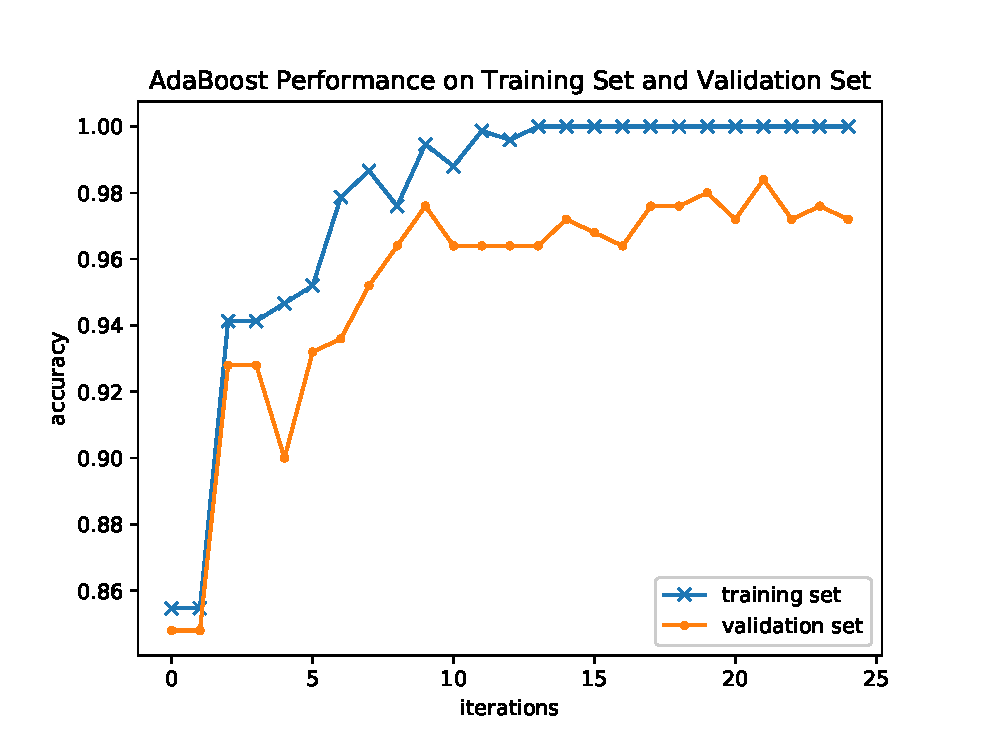
\includegraphics[width=\columnwidth]{adaboost_accuracy}
		% Create a subtitle for the figure.
		\caption{AdaBoost performance on both training set and validation set.}
		% Define the label of the figure. It's good to use 'fig:title', so you know that the label belongs to a figure.
		\label{fig:adaboost_accuracy}
		\end{center}
	\end{figure}

	% This is how you define a table: the [!hbt] means that LaTeX is forced (by the !) to place the table exactly here (by h), or if that doesnt work because of a pagebreak or so, it tries to place the table to the bottom of the page (by b) or the top (by t).
	\begin{table}[!hbt]
		% Center the table
		\begin{center}
		% Title of the table
		\caption{Face Classification Report}
		\label{tab:adaboost_report}
		% Table itself: here we have two columns which are centered and have lines to the left, right and in the middle: |c|c|
		\begin{tabular}{|c|c|c|c|c|}
			% To create a horizontal line, type \hline
			\hline
			% To end a column type &
			% For a linebreak type \\
			  & precision & recall & f1-score & support \\
			\hline
			nonface & 0.98 & 0.97 & 0.97 & 125 \\
			\hline
			face & 0.97 & 0.98 & 0.97 & 125 \\
			\hline
			avg / total & 0.97 & 0.97 & 0.97 & 250\\
			\hline
		\end{tabular}
		\end{center}
	\end{table}

    %                precision    recall  f1-score   support
    %     nonface       0.98      0.97      0.97       125
    %        face       0.97      0.98      0.97       125
    % avg / total       0.97      0.97      0.97       250

	% If you have questions about how to write mathematical formulas in LaTeX, please read a LaTeX book or the 'Not So Short Introduction to LaTeX': tobi.oetiker.ch/lshort/lshort.pdf


\section{Conclusion}
    In this experiment, we implement a AdaBoost model to solve face classification problem. We train the model on training set and evaluate it on validation set. The result show that AdaBoost performs well in this problem.
    This process gives us a better understanding of the AdaBoost algorithm and how to combine the theory with the actual project. That let us experience the complete process of machine learning.



% Your document ends here!
\end{document}